\section{Evaluation}
\label{sec:evaluation}
\sisetup{exponent-mode = scientific}

The first part of the evaluation will deal with the adjustments and what can be inferred from them.
Following the main measurements will be shown which get evaluated later on. The last part of the evaluation will deal with the Parratt algorithm.
\subsection{Adjustments}

\subsubsection{Detector Scan}
In figure \ref{fig:detector_scan} the reflectivity of the sample is plotted against the incident angle for the detector scan.
Furthermore a fit of the form 
\begin{equation*}
  b+\frac{a\cdot1.0 }{ \sigma\cdot \sqrt{2 \cdot \pi}} \cdot \exp\left(-0.5 \cdot \left(\frac{x - \mu}{\sigma}\right) ^ 2\right)  
\end{equation*} 
is performed, which corresponds to a Gaussian fit with two additional parameters $a$ and $b$.
The parameters are given in table \ref{tab:detector_scan}.
With help of this function the FWHM and the maximum of the intensity can be calculated.
The FWHM is marked in figure \ref{fig:detector_scan} as well.
The values are $\text{FWHM} = \qty{0.144}{\degree}$ and $\text{I}_\text{max}=\num{1.110(0.020)e6}$.


\begin{table}[H]
  \centering
  \caption{Parameters of the fit shown in figure \ref{fig:detector_scan}.}
  \label{tab:detector_scan}
  \sisetup{table-format=1.1, per-mode=reciprocal}
  \begin{tblr}{
      colspec = {S[table-format=3.0] S[table-format=2.1] S},
      row{1} = {guard, mode=math},
      % vline{4} = {2}{-}{text=\clap{$\pm$}},
      }
    \toprule
    \mu & \sigma & a & b \\
    \midrule
    % \qty{-6.604 1e-3}{\degree} & \qty{61.725 1e-3}{\degree} & \qty{171380.529}{\degree} & 2628.667 \\
    \qty{-0.0007(0.0007)}{\degree} & \qty{0.0617(0.0008)}{\degree} & \qty{1.714(0.022)e5}{\degree} & \num{3(4)e3} \\
    \bottomrule
  \end{tblr}
\end{table}

\begin{figure}[H]
  \centering
  \includegraphics{build/detector_scan_1.pdf}
  \caption{Plot of the intensity against the incident angle resulting from the detector scan.}
  \label{fig:detector_scan}
\end{figure}

\subsubsection{Z-Scan}
The scan gives insight into the width of th x-ray beam. From figure \ref{fig:z_scan} the beam width can
be estimated by measuring the minimum width of the crossing between minimum and maximum values.
The width is $\qty{0.64}{\milli\meter}$.
\begin{figure}[H]
  \centering
  \includegraphics{build/z_scan_1.pdf}
  \caption{Intensity against the z position of the sample for the z-scan.}
  \label{fig:z_scan}
\end{figure}

\subsubsection{Rockingscan}\label{sec:rockingscan}
Figure \ref{fig:rockingscan} shows the rockingscan. The rockingscan is used to determine the geometry angle. 
The geometry angle is the angle, where the intensity drops to zero. In this case the angle range is to small, 
so that the relevant area is not visible. Because of that it is assumed, that 
the scan is linearly on the left and right from the maximum. A linear fit is performed on both sides.
The interval between the intersections of these fits with the x-axis should be equal to $2\cdot\alpha_\text{g}$.

\begin{figure}[H]
  \centering
  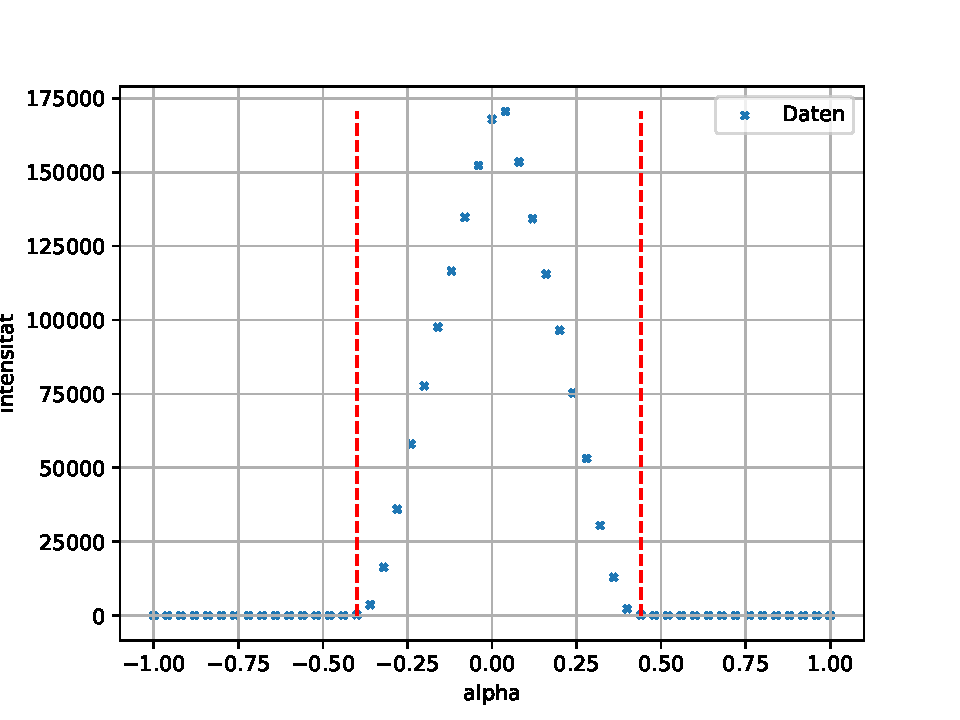
\includegraphics{build/rockingscan.pdf}
  \caption{The Plot displays the rockingscan and how the geometry angle is measured}
  \label{fig:rockingscan}
\end{figure}

The measured geometry angle is $\alpha_g=\qty{1.296}{\degree}$. 
With equation \eqref{eqn:geometry_factor} and values $D=\qty{2}{\cm}$, the width of the sample, and $d_0=\qty{0.64}{\milli\meter}$ determined through the z-scan the 
theoretical geometry angle is calculated as $\alpha_\text{g}=\qty{1.834}{\degree}$.




\subsection{Measurement of Reflectivity and Background}
Figure \ref{fig:basic_measurement} shows the reflectivity against the incident angle for the measurement of the sample.
Additionally the background measurement is shown which is used to correct the results of the previous measurement.
The correction is performed by subtracting the background measurement from the measurement of the sample.
In the following diagrams the reflectivity instead of the intensity is shown. 
The connection between reflectivity and intensity is given through
\begin{equation}
  R=\frac{I}{5\cdot I_\text{max}}.
\end{equation}
The reason for that is that the intensity is measured over \qty{5}{\second}.

\begin{figure}[H]
  \centering
  \includegraphics{build/basic_reflectivity_curves.pdf}
  \caption{Reflectivity against the incident angle. The three curves show the measurement of the sample 
  included, the sample excluded for determination of background and the first measurement corrected with the 
  background measurement.}
  \label{fig:basic_measurement}
\end{figure}


\subsection{Comparison of reflectivity from fresnel theory and corrected by geometry factor}
Figure \ref{fig:advanced_curves} displays the reflectivity which was just corrected for background and the reflectivity which is also corrected with the geometry factor.% as it can be calculated with formula \eqref{}.
The third curve is the theoretical fresnel reflectivity for one flat silicon layer calculated with formula \eqref{eqn:fresnel}. 
% Formula \eqref{eq:fresnel_approximation} is only valid for angles above the critical angle which 
% explains the reduced angle range in figure \ref{fig:advanced_curves}.
\begin{figure}[H]
  \centering
  \includegraphics{build/advanced_curves.pdf}
  \caption{Reflectivity against the incident angle for the measurement which has been corrected for the background. On more curve shows the correction with the geometry factor. Both curves are compared to the theoretical curve calculated with fresnel formulas.}
  \label{fig:advanced_curves}
\end{figure}


\subsection{Comparison of measured reflectivity and Parratt algorithm}
To extract meaningful results from the measured curve, the Parratt algorithm is used. 
The Parratt algorithm contains adjustable parameters as given in table \ref{tab:parratt_params}. 
To adjust these parameters a parameter search is performed. A common grid search is not possible, because 7 parameters need to be optimized, which leads
to more parameter combinations than can be tested in an acceptable period of time. 
Therefor a TPE sampler is used, which can handle high dimensional parameter searches. The TPE sampler is an improved version of a random sampler 
and can determine the next parameter combination that will likely produce good result based on the results of the previous parameter combinations.
The python package \texttt{optuna}\cite{v44:optuna} provides an implementation of the TPE and is used for this evaluation.
To make the TPE work, an appropriate type of loss function/distance metric needs to be determined between the measured curve and the calculated curve from the Parratt algorithm.
In this case 
\begin{equation*}
  d=\sum_i \left|\ln\left(\frac{1}{\text{measured}_i+c}\right)-\ln\left(\frac{1}{\text{parratt}_i+c}\right) \right|
\end{equation*}
proves to be a good distance measure. It takes into account that the data spans several magnitudes. 
The constant $c$ prevents divisions by zero in the program.
The resulting parameters determined through the parameter search are given in table \ref{tab:parratt_params}.
\begin{table}[H]
  \centering
  \caption{Parameters of the fit shown in figure \ref{fig:detector_scan}.}
  \label{tab:parratt_params}
  % \sisetup{table-format=1.1, per-mode=reciprocal}
  % \begin{tblr}{S[table-format=3.0],S[table-format=2.1]}
    \begin{tabular}{c S[table-format=1.3e-2] r}
    \toprule
     \text{layer thickness} & 8.551e-08\,m &\\
     $\delta_\text{Si}$     & 7.672e-06 \\
     $\delta_\text{Po}$     & 1.124e-06 \\
     $\beta_\text{Si} $     & 8.779e-08 \\
     $\beta_\text{Po} $     & 1.109e-08 \\
     $\sigma_\text{Si}$     & 7.320e-10\,m \\
     $\sigma_\text{Po}$     & 9.842e-10\,m \\
    \bottomrule
  \end{tabular}
\end{table}
Besides the parameters shown in the table, the wavelength is needed which is $\lambda=\qty{1.54e-10}{\m}$.
The result of the Parratt algorithm is shown in figure \ref{fig:parratt} next to the measurement that is corrected with the geometry factor. 
\begin{figure}[H]
  \centering
  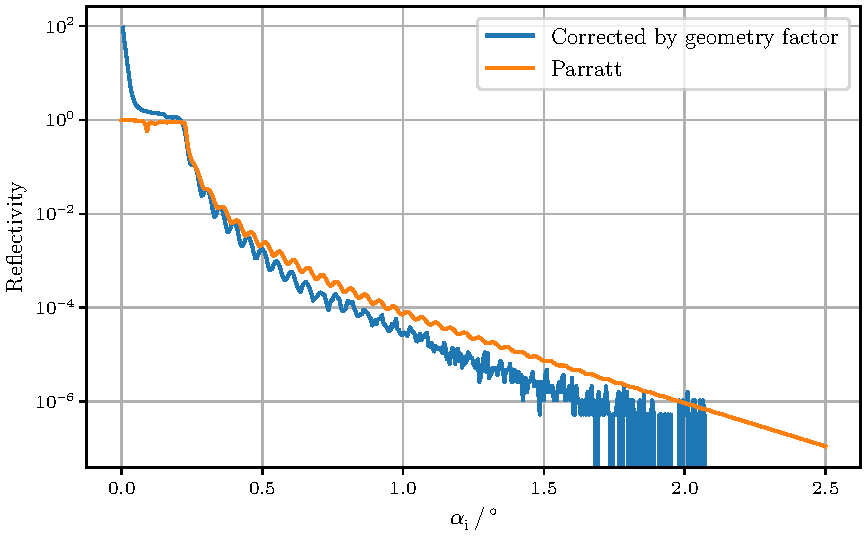
\includegraphics{build/parrat_comparison.pdf}
  \caption{Comparison of measured reflectivity corrected with geometry factor and calculated reflectivity with Parratt algorithm.}
  \label{fig:parratt}
\end{figure}

\subsection{Layer thickness and critical angle}
The layer thickness is calculated with formula \eqref{eqn:thickness}. 
The angles between consecutive minimas in the Kiessig oscillations are calculated with \texttt{find\_peaks} from \texttt{scipy.signal}.
The mean angle will be used for calculating the thickness. Furthermore only a fraction of the measured curve
is used where minima can be determined reliably.
The resulting thickness is $z=\qty{8.82(0.23)e-8}{\m}$.
The critical angle $\alpha_c$ can be calculated with \eqref{eqn:critical_angle} and the dispersions from the Parratt optimization which leads to
\begin{align*}
  \alpha_\text{c,Si} &=\qty{0.224}{\degree}~\text{and}\\
  \alpha_\text{c,Pol}&=\qty{0.0860}{\degree}.\\
\end{align*}





% \begin{table}
%   \centering
%   \caption{}
%   \label{}
%   \begin{tabular}{cc}
%     \toprule
%     Thickness
%     \midrule

%     \bottomrule
%   \end{tabular}
% \end{table}
  









































% \begin{figure}
%   \centering
%   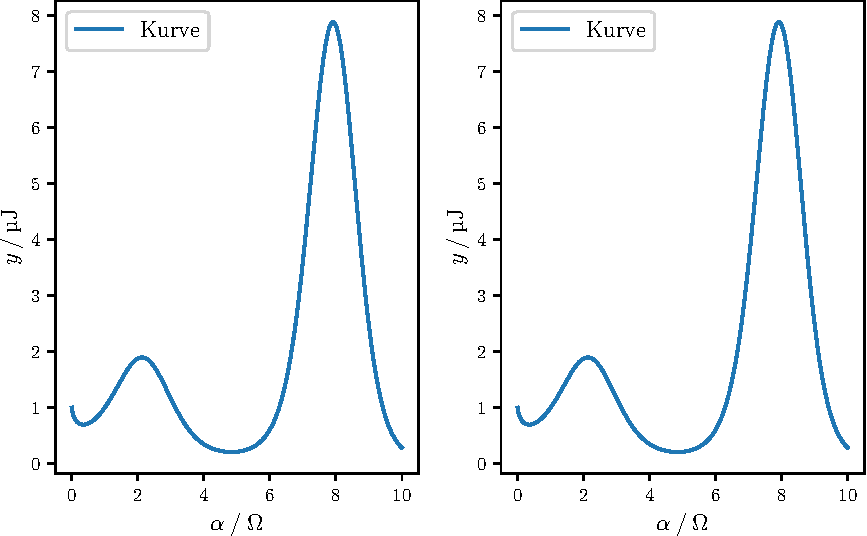
\includegraphics{plot.pdf}
%   \caption{Plot.}
%   \label{fig:plot}
% \end{figure}

% \begin{table}
%   \centering
%   \caption{Eine Beispieltabelle mit Messdaten.}
%   \label{tab:tabelle}
%   \sisetup{table-format=1.1, per-mode=reciprocal}
%   \begin{tblr}{
%       colspec = {S[table-format=3.0] S[table-format=2.1] S},
%       row{1} = {guard, mode=math},
%       vline{4} = {2}{-}{text=\clap{$\pm$}},
%     }
%     \toprule
%     U \mathbin{/} \unit{\volt} & I \mathbin{/} \unit{\micro\ampere} & \SetCell[c=2]{c} N \mathbin{/} \unit{\per\second} & \\
%     \midrule
%     360 & 0.1 & 98.3 & 0.9 \\
%     400 & 0.2 & 99.8 & 1.0 \\
%     420 & 0.2 & 99.1 & 0.9 \\
%     \bottomrule
%   \end{tblr}
% \end{table}

% Siehe \autoref{fig:plot} und \autoref{tab:tabelle}!
